%% Coherence sweet spots across superconducting qubit architectures
%%
%% VENUE: arXiv preprint only (author's decision, 2026-10-01). No journal submission.
%% SciPost.cls / SciPost_bibstyle.bst are used purely as a single-column layout; the
%% journal header, submission box and referee line numbers are deliberately absent.
%% main.tex is the earlier IEEE TQE version, frozen; this file is the live source.
%%
%% Build:           tectonic -X compile preprint.tex
%% arXiv bundle:    python make_arxiv.py   (see ARXIV.md)
%%
%% EVERY number in this paper is traceable to data/headline_provenance_ledger.csv,
%% which 05_summary.ipynb regenerates and asserts. If you change a number here,
%% change it there first and let the ledger verify it.
\documentclass{SciPost}
\fancyhead{}                          % no journal header: this is a preprint
\renewcommand{\headrulewidth}{0pt}

% The SciPost class's template sets \binoppenalty=\relpenalty=10000 to forbid line breaks
% inside inline math. This paper has dense inline math in single-column text, and that
% setting forces six overfull lines, so it is relaxed to discourage-but-allow.
\binoppenalty=700
\relpenalty=500

\hypersetup{
    colorlinks,
    linkcolor={red!50!black},
    citecolor={blue!50!black},
    urlcolor={blue!80!black}
}

\usepackage[bitstream-charter]{mathdesign}
\urlstyle{sf}
\usepackage{booktabs,siunitx,microtype}
% Upright micro sign. Under XeTeX with mathdesign's T1 Charter, siunitx's default micro lands on
% T1 slot 181, which is "t-cedilla": every microsecond printed as "ţs". TS1 slot 181 is the
% real micro sign, and works under pdfLaTeX (arXiv) too.
\providecommand{\upmu}{\text{\fontencoding{TS1}\selectfont\char181}}
\DeclareSIPrefix{\micro}{\upmu}{-6}
\usepackage{xurl}   % break long URLs
\emergencystretch=1.5em   % absorbs the few unbreakable inline-math runs

\begin{document}

\begin{center}{\Large \textbf{\color{scipostdeepblue}{
Coherence sweet spots are frequency minima in disguise:\\
Metric sensitivity in transmon and fluxonium design spaces
}}}\end{center}

\begin{center}\textbf{
Ishita Bera\textsuperscript{1$\star$}
}\end{center}

\begin{center}
% Affiliation as confirmed for the IEEE version. Change only on the author's say-so.
{\bf 1} Independent researcher
\\[\baselineskip]
$\star$ \href{mailto:ishitabera4@gmail.com}{\small ishitabera4@gmail.com}
\end{center}

\section*{\color{scipostdeepblue}{Abstract}}
{\bfseries\boldmath
Dielectric loss is well known to scale with transition frequency, implying that a
lower-frequency qubit relaxes more slowly at fixed quality factor. We show that this has a
stronger consequence for design studies than is usually acknowledged. Under a common noise
model, $\log T_2$ over the transmon $(E_J,E_C)$ plane correlates with $\log f_{01}$ at
$r=-0.9999$ within the transmon regime, while over the fluxonium $(E_J,E_L)$ plane the
correlation is $r=-0.9973$. Because each parameter plane effectively reduces to a single degree of
freedom, the transition frequency, a raw $T_2$ maximum primarily identifies the
lowest-frequency corner of the swept domain rather than an intrinsic optimal design. Indeed,
both of our initial headline optima occur at grid-edge points outside any usable frequency band.

Controlling for frequency changes these conclusions. For the transmon, we find no interior
optimum in $E_J/E_C$ at fixed $f_{01}$. $T_2$ varies by only 4.8\% across a tenfold range in
$E_J/E_C$, while the anharmonicity decreases by a factor of 7.3. Charge insensitivity is
therefore obtained primarily at the cost of gate speed rather than through improved coherence,
and any reported optimum depends on the imposed regime boundary.

The fluxonium has a genuine interior optimum once second-order
$1/f$ flux dephasing is included, but it occurs at frequencies of only 10--73\,MHz, where
$\bar n_{\mathrm{th}}=4$--$32$. For the cross-architecture comparison, there is no single
answer: the fluxonium/transmon ratio spans ${\sim}500\times$ across defensible metrics, while
at matched frequency the $T_2$ advantage reverses to a median $0.86\times$ across the
literature noise band. A lab-frame pulse simulation yields a $36$--$58\times$ advantage in
gate count, excluding both analytic bounds: the fluxonium drive couples
$10.2\times$ more strongly to its leakage transition than to its qubit transition.\par}

\vspace{\baselineskip}
\noindent\rule{\textwidth}{1pt}
\tableofcontents
\noindent\rule{\textwidth}{1pt}
\vspace{10pt}

\section{Introduction}

Superconducting qubit design is routinely discussed in terms of \emph{sweet spots}:
bias points at which the transition frequency is stationary with respect to a noise
coordinate, so that first-order dephasing vanishes. The transmon has charge sweet spots
at integer and half-integer offset charge, and its exponentially suppressed charge dispersion
keeps it nearly insensitive in between~\cite{koch2007}; the fluxonium achieves it at
half a flux quantum, where $\partial\omega_{01}/\partial\Phi = 0$ by
symmetry~\cite{nguyen2019}. Both are then said to have a coherence sweet
spot in \emph{design} space as well, and the point of best modeled $T_2$ over a swept
parameter plane is reported as an optimum.

This paper argues that the second usage does not survive scrutiny, and that the error is
systematic rather than incidental. We address three questions:

\begin{itemize}
\item[\textbf{Q1}] Where are the coherence optima across the transmon $(E_J, E_C)$ and
      fluxonium $(E_J, E_C,\allowbreak E_L, \Phi)$ design spaces?
\item[\textbf{Q2}] Which noise channel dominates where?
\item[\textbf{Q3}] Does the fluxonium's flux sweet spot buy more robustness than the
      transmon's charge insensitivity, and at what cost?
\end{itemize}

Our central methodological claim is that Q1 and Q3 cannot be answered without controlling
for the transition frequency, and that once controlled the conventional answers change sign
or dissolve. Our central negative result is that the fluxonium's coherence advantage at
matched frequency does not survive the uncertainty in the noise amplitudes that the model
itself assumes.

Figure~\ref{fig:summary} summarizes the study. All results are model-based estimates under
literature noise amplitudes. They are not predictions of device performance, and
Section~\ref{sec:calibration} quantifies how far they sit from measurement.

\begin{figure}[t]
\centering
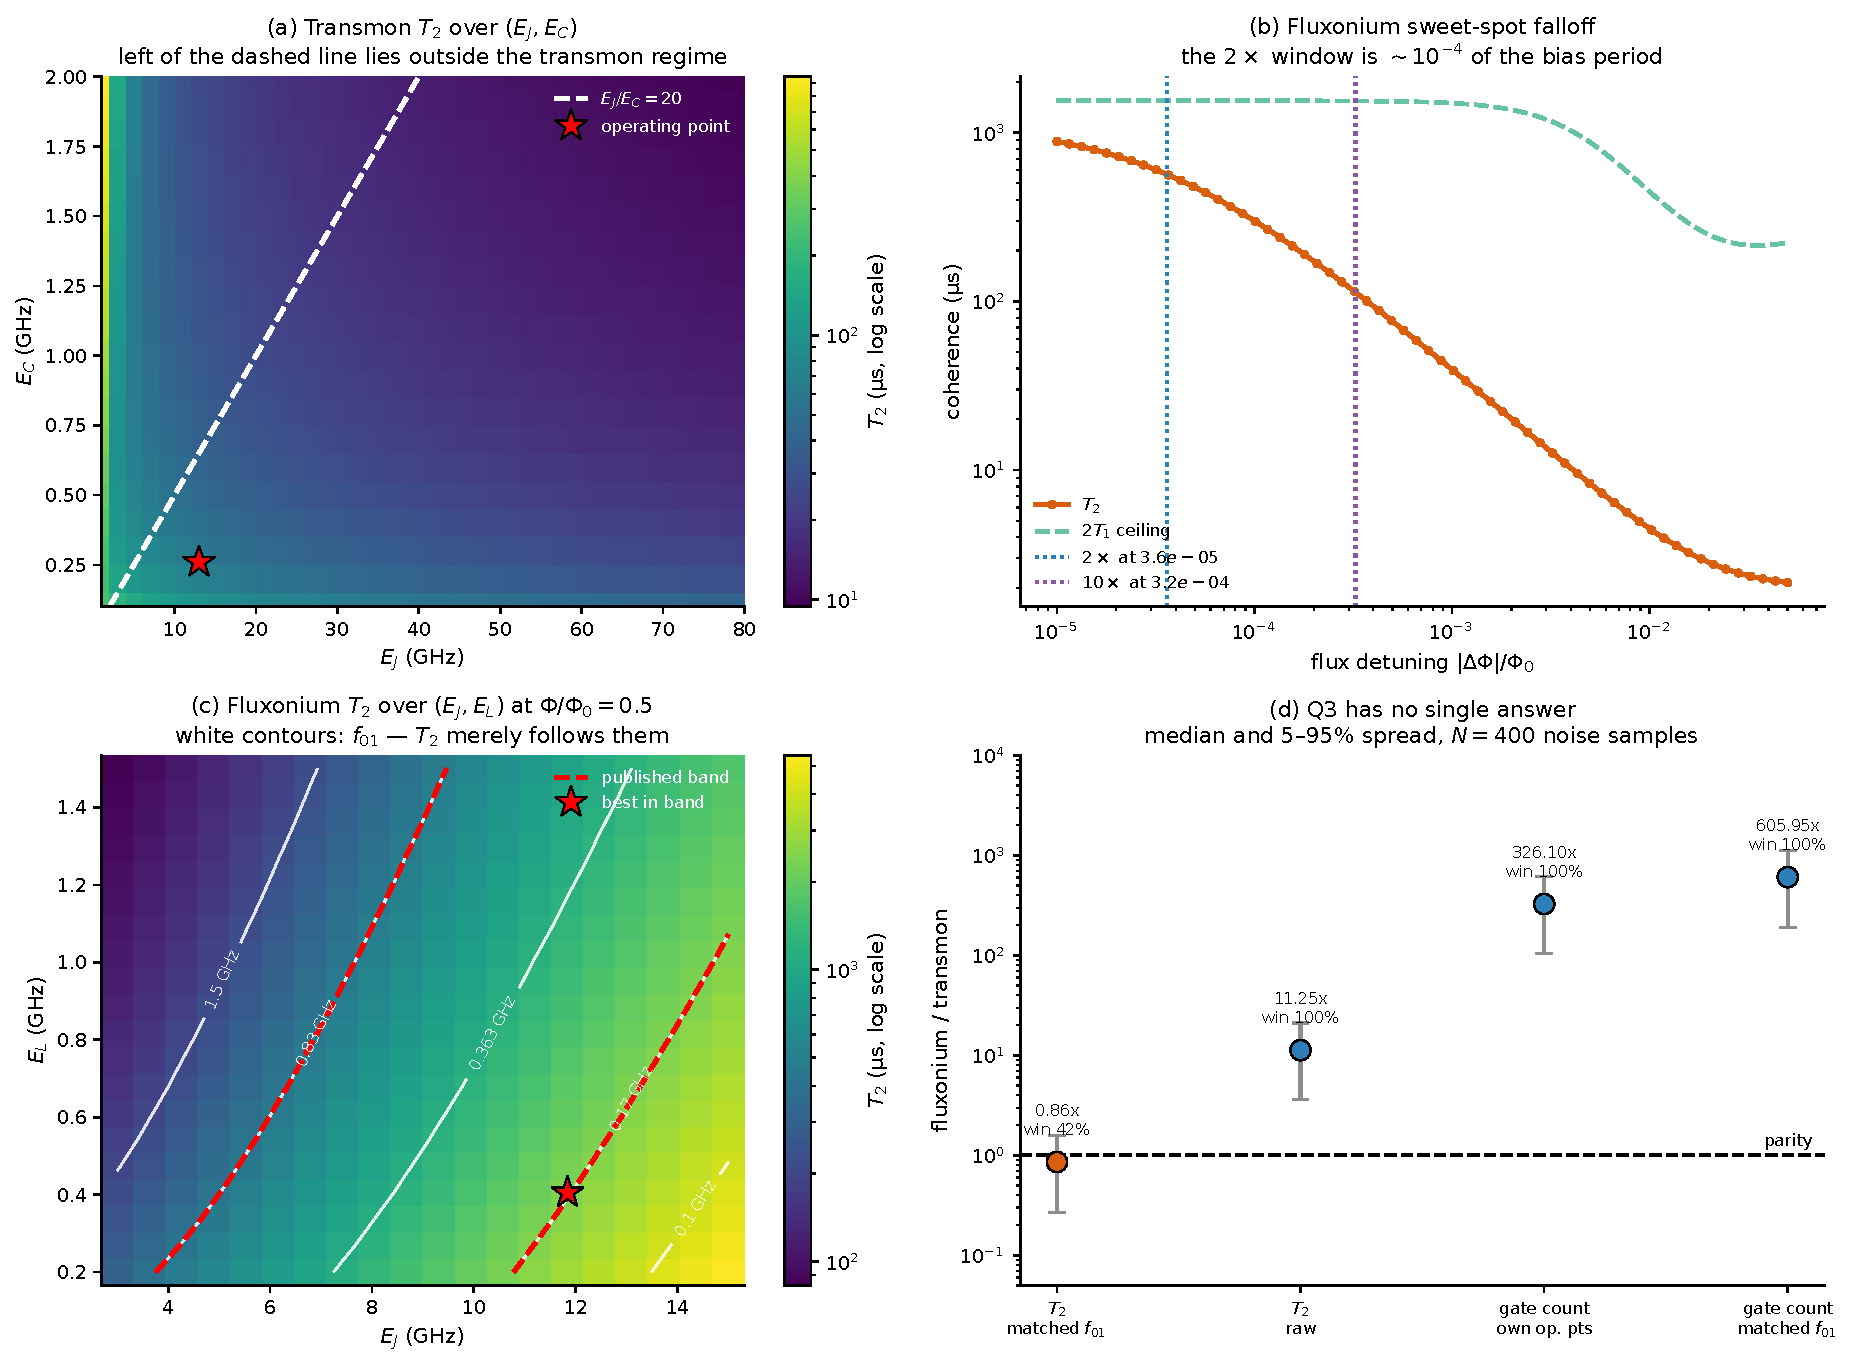
\includegraphics[width=\textwidth]{figures/summary_figure.pdf}
\caption{The study in four panels. (a) Transmon $T_2$ over $(E_J, E_C)$ at $n_g = 0$; left of
the dashed line ($E_J/E_C < 20$) lies outside the transmon regime, and its numbers are not
transmon results. (b) The
fluxonium sweet-spot falloff on a log-detuning axis, with the $2T_1$ ceiling and the two-
and tenfold loss points; on a linear flux axis the entire collapse hides inside the first
0.1\% of the plot. (c) Fluxonium $T_2$ over $(E_J, E_L)$ at half flux, with $f_{01}$ contours
in white --- the $T_2$ structure merely follows them, which is the confound this paper is
about. (d) The Q3 answer under each metric, with the 5--95\% spread over $N=400$ noise-amplitude
draws; orange marks the metrics in which the fluxonium wins fewer than 90\% of samples.}
\label{fig:summary}
\end{figure}

\section{Related Work and Contribution}

\subsection{What is already established}

The frequency scaling on which we build is not a new idea. Dielectric loss at surfaces and
interfaces, commonly attributed to two-level-system defects, is a major relaxation mechanism in
superconducting qubits; in 3D transmons the relaxation rate scales approximately with the
surface participation of lossy dielectrics~\cite{wang2015}. At fixed effective quality factor, $\Gamma_1\propto\omega_{01}$, so a
lower-frequency qubit relaxes more slowly. Design-space optimization under explicit noise models
is likewise established: Papi\v{c} \emph{et al.} identify optimal transmon parameter ranges using
comprehensive noise modeling that includes charge-parity effects~\cite{papic2024}, while Ram
\emph{et al.} present a staged framework spanning circuit design, spectral analysis, and
calibration for both architectures~\cite{ram2025}. Experimentally, fluxonium coherence has
advanced well beyond the devices against which we calibrate our model: Somoroff \emph{et al.}
report $T_2^* = 1.48$\,ms together with an average gate fidelity of
$0.99991$~\cite{somoroff2023}.

Two works are sufficiently close to the present study to warrant more precise comparison.
McRae \emph{et al.}~\cite{mcrae2021} argue that coherence metrics cannot yet be reliably
compared across measurements, devices, and laboratories because temporal fluctuations, TLS
dynamics, and incompletely reported experimental conditions can make the claimed differences
unreliable. Their concern is experimental reproducibility. The present paper develops a modeling
analog of that argument: a comparison extracted from a swept design space is likewise
unreliable unless both the controlled variable and the figure of merit are specified alongside
the reported value.

Lange \emph{et al.}~\cite{lange2025} directly compare transmon and fluxonium lattices and
conclude that fluxonium architectures may show lower cross-talk when designed for similar gate
speeds and fidelities, a matching they argue from coupling strengths in published
two-qubit-gate experiments. Their figures of merit are residual $ZZ$ cross-talk and
state localization rather than coherence. Our work is complementary: it applies the same
principle of controlled comparison to coherence and asks how the conclusion changes when
transition frequency is held fixed.

\subsection{Contribution}

Our contribution is not the frequency scaling itself, but its consequence for how design studies
are interpreted:

\begin{enumerate}
\item We quantify the frequency confound in both architectures, finding $|r|>0.99$ between
      modeled $\log T_2$ and $\log f_{01}$ across the relevant design planes. As a result, a raw
      $T_2$ optimum can primarily reflect the lowest-frequency boundary of the sweep rather than
      an intrinsic design optimum.
\item We show that the transmon's gate-count optimum within the 3--6\,GHz band is pinned to the
      imposed regime threshold across eight thresholds spanning $E_J/E_C=15$--$60$. The
      substantive choice is therefore the threshold itself, rather than the subsequent
      optimization within that domain.
\item We show that including second-order $1/f$ flux dephasing produces an interior fluxonium
      optimum that is absent from a first-order treatment.
\item We show that the transmon--fluxonium coherence comparison varies substantially across
      defensible figures of merit, and we narrow the gate-count comparison, the one most
      sensitive to its assumptions, to 36--58$\times$ by direct pulse simulation.
\end{enumerate}

We are not aware of prior work that explicitly examines how strongly the transmon--fluxonium
coherence comparison depends on the chosen metric. This rests on the survey above, which is
not exhaustive; the individual ingredients are known, and the claim concerns their combination.
Our contribution is to show this dependence
and how controlling for transition frequency changes the resulting design conclusions.

\subsection{A limitation of the present comparison}

Matching $f_{01}$ removes the dominant confound but not all of it. Dielectric loss also depends
on geometry and surface participation, which differ between architectures and which a
Hamiltonian-level model does not capture~\cite{wang2015}, and real devices fluctuate in ways no
static model represents~\cite{mcrae2021}. Frequency matching is necessary, not sufficient, and
our matched-frequency numbers should be read as removing one large confound rather than as a
fully controlled experiment.

A second limitation follows from the matching itself. The fluxonium's sweet-spot frequency lies
below the transmon band, so the matched transmons sit at 0.5--2\,GHz with
$E_J/E_C = 325$--$5050$ and $|\alpha| \approx \SI{10}{\mega\hertz}$, far outside the design
envelope adopted in Section~\ref{sec:transmon}. Because the modeled transmon $T_2$ at fixed
$f_{01}$ is nearly independent of $E_J/E_C$, this does not bias the $T_2$ comparison, but it means
the matched transmons are not usable qubits, and gate-based metrics at matched frequency should
not be read as device comparisons.

\section{Model and Conventions}

\subsection{Noise channels}

Coherence is estimated using \texttt{scqubits}~\cite{groszkowski2021}. Independent relaxation and
dephasing rates are combined as
\begin{equation}
\frac{1}{T_2} = \frac{1}{2T_1} + \sum_k \frac{1}{T_{\phi,k}},
\label{eq:rates}
\end{equation}
with noise channels selected separately for each architecture. The fixed-frequency transmon
considered here contains no flux-tunable loop, so $1/f$ flux dephasing is not included. In the
fluxonium model considered here, the inductive shunt removes the dependence on offset charge
entirely, so charge dephasing is not included. Table~\ref{tab:channels} summarizes the channel
assignments.

\begin{table}[t]
\caption{Noise channels by architecture.}
\label{tab:channels}
\centering
\begin{tabular}{@{}llcc@{}}
\toprule
Channel & \texttt{scqubits} method & Transmon & Fluxonium\\
\midrule
Dielectric loss ($T_1$)   & \texttt{t1\_capacitive}          & \checkmark & \checkmark\\
Quasiparticle ($T_1$)     & \texttt{t1\_quasiparticle\_tunneling} & --         & \checkmark\\
$1/f$ flux, 1st order     & \texttt{tphi\_1\_over\_f\_flux}  & --         & \checkmark\\
$1/f$ flux, 2nd order     & \emph{this work}                 & --         & \checkmark\\
Charge / offset           & \texttt{tphi\_1\_over\_f\_ng}    & \checkmark & --\\
Critical current          & \texttt{tphi\_1\_over\_f\_cc}    & \checkmark & \checkmark\\
\bottomrule
\end{tabular}
\end{table}

We use $Q_{\mathrm{cap}}=10^6$, $A_{n_g}=10^{-4}$, $A_\Phi=10^{-6}\,\Phi_0$, and
$A_{\mathrm{cc}}=10^{-7}$. The chosen flux-noise amplitude, $A_\Phi=1\,\upmu\Phi_0$, is slightly below
the values measured on flux-sensitive devices, $1.4\,\upmu\Phi_0$~\cite{yan2016} and
$1.8\,\upmu\Phi_0$~\cite{nguyen2019}, and is therefore optimistic. Temperature, quasiparticle density, and the $1/f$ cutoffs are
otherwise taken from the \texttt{scqubits} defaults ($T=\SI{15}{\milli\kelvin}$,
$x_{\mathrm{qp}}=3\times10^{-6}$, $t_{\mathrm{exp}}=\SI{10}{\micro\second}$) and are recorded with
every result because these parameters materially affect the predicted coherence times.

\subsection{Second-order flux dephasing}

\texttt{scqubits} evaluates $1/f$ dephasing to first order in the sensitivity
$\partial\omega_{01}/\partial\lambda$. At an exact flux sweet spot,
$\partial\omega_{01}/\partial\Phi=0$, so the first-order dephasing rate vanishes and the
corresponding calculated dephasing time diverges~\cite{groszkowski2021}. The leading flux
sensitivity at half flux is therefore second order. We include the second-order contribution
using the expression employed for fluxonium by Nguyen \emph{et al.}~\cite{nguyen2019}, following
Ithier \emph{et al.}~\cite{ithier2005}:
\begin{equation}
\Gamma_\Phi^{(2)} = \left|\frac{\partial^2\omega_{01}}{\partial\Phi^2}\right| A_\Phi^2 .
\label{eq:secondorder}
\end{equation}
Equation~\eqref{eq:secondorder} contains no logarithmic factor under this convention. Alternative
treatments introduce factors involving $|\ln(\omega_{\mathrm{low}}t_{\mathrm{exp}})|$, producing
substantial quantitative changes in the inferred dephasing time. Rather than selecting among these
conventions implicitly, we report the associated sensitivity explicitly
(Section~\ref{sec:limitations}). The required curvature is evaluated using Richardson
extrapolation, since a simple central difference remains 4--10\% from its converged value in the
deepest-well part of the scan ($E_J=40$--\SI{45}{\giga\hertz}, $E_L=\SI{0.2}{\giga\hertz}$),
though within 0.2\% at the interior optima of Section~\ref{sec:fluxonium}.

\subsection{A declared modeling choice}

Passing $Q_{\mathrm{cap}}$ explicitly replaces the \texttt{scqubits} default frequency-dependent
quality factor, $Q_{\mathrm{cap}}(\omega)\propto\omega^{-0.7}$~\cite{smith2020}, with a constant
value. At the fluxonium sweet spot, these two assumptions change the calculated $T_1$ by a factor
of $7.1$, making this the largest single modeling choice in the study. The resulting uncertainty
is not symmetric: Nguyen \emph{et al.} fit their measured $T_1$-versus-frequency dependence with
$\tan\delta_C\propto\omega^{0.15}$, and at $f_{01}=\SI{0.363}{\giga\hertz}$ the constant-$Q$ model
lies $1.52\times$ from their measured scaling, compared with $4.7\times$ for the \texttt{scqubits}
default. That exponent was fit jointly with thermal effects and is not an independent measurement
of the loss tangent, but it favors the constant-$Q_{\mathrm{cap}}$ model, which we therefore
retain as the more conservative and better-supported choice, while stating the assumption
explicitly.

\section{Validation}
\label{sec:validation}

Forty-four checks validate the numerical pipeline before the results presented below are
generated. These tests include exact Hamiltonian symmetries to machine precision, basis-size
convergence, analytic limits from Koch \emph{et al.}~\cite{koch2007}, and, in several cases,
comparison with published data from experimental devices.

The strongest analytic benchmark is Koch \emph{et al.}'s worked charge-dephasing example. For
$E_J=\SI{30}{\giga\hertz}$, $E_C=\SI{0.35}{\giga\hertz}$, and $A=10^{-4}$, they report
$T_2\sim\SI{8}{\second}$. Substituting our computed charge dispersion into their Eq.~(5.9) gives
$T_2=\SI{8.75}{\second}$. At $E_J/E_C=50$, the maximum charge-dispersion derivative is $0.830$
times their asymptotic value of $1.5\times10^{-4}E_C$, consistent with the asymptotic expression
being approached from below.

Against Manucharyan \emph{et al.}~\cite{manucharyan2009}, the lowest two transitions at
$\Phi_{\mathrm{ext}}=0$ are reproduced to better than $0.7\%$ for each of the paper's three
published parameter sets. A single four-parameter fit additionally reproduces all six digitized
transition lines across two flux biases with an RMS error of $\SI{0.0102}{\giga\hertz}$. The three
published parameter sets---the rounded main-text values and two Table~I least-squares fits---produce
a $9.5\%$ spread in $f_{01}$ at the flux sweet spot. Agreement quoted only against the rounded
main-text parameters would therefore overstate the experimental constraint.

The third transition at $\Phi_{\mathrm{ext}}=0$ is excluded from this comparison for a physical
rather than numerical reason. Its bare frequency lies only 0.14--0.36\,GHz from the junction-array
mode placed at $\SI{10.78}{\giga\hertz}$ by Manucharyan's extended model, while the 0--3 coupling,
which we compute from that model, is approximately $\SI{0.53}{\giga\hertz}$. The coupling therefore
exceeds the detuning by a factor of 1.5--3.7, placing the transition in a strongly hybridized regime
that cannot be captured by the bare-circuit model. Explicit diagonalization of the fluxonium coupled
to both array modes confirms that this discrepancy is concentrated near $\Phi_{\mathrm{ext}}=0$. The
dressed $f_{01}$ shifts by $-16\%$ there, but by only $-0.43\%$ at the flux sweet spot, where the
coherence calculations in this study are performed. This residual shift is smaller than the $9.5\%$
spread produced by the paper's own published parameter sets.

Finally, the second-order channel in Eq.~\eqref{eq:secondorder} is the only physical contribution
implemented here rather than inherited from established tooling, so we check it against an
independent published evaluation rather than against its defining equation alone. Nguyen
\emph{et al.}, using the same expression and their measured $A_\Phi=1.8\,\upmu\Phi_0$, state that
the second-order limit exceeds $\SI{10}{\milli\second}$ for all of their qubits~\cite{nguyen2019}.
Evaluated for their nine devices at the same amplitude, our implementation gives
$T_{\phi}^{(2)}=15$--$\SI{804}{\milli\second}$, consistent with that statement.

\section{The Transmon Design Plane}
\label{sec:transmon}

We sweep $E_J \in [1, 80]$, $E_C \in [0.1, 2.0]$\,GHz at $n_g = 0$ and $n_g = 0.25$
(800 points each), and refine to a $65\times53$ grid over $E_J \in [4,20]$,
$E_C \in [0.08, 0.6]$\,GHz.

\subsection{The confound}

Within the transmon regime $E_J/E_C \ge 20$, $\mathrm{corr}(\log T_2, \log f_{01}) = -0.9999$.
The plane contains one degree of freedom, not two. The reason is structural rather than
numerical: dielectric loss dominates $T_1$ everywhere in the regime, with
$\Gamma \propto |\langle 0|\hat n|1\rangle|^2 S(\omega_{01})$. Since
$|\langle 0|\hat n|1\rangle|^2 \propto \sqrt{E_J/E_C}$ and $S \propto E_C$, the rate goes as
$\sqrt{E_JE_C} \propto \omega_{01}$---a function of frequency alone. Consequently the best
$T_2$ point of the swept plane, \SI{187}{\micro\second} at $E_J = 3.03$,
$E_C = \SI{0.10}{\giga\hertz}$, sits at the corner of the admissible domain---the smallest
$E_C$ on the grid and the smallest $E_J$ satisfying $E_J/E_C \ge 20$---at
$f_{01} = \SI{1.45}{\giga\hertz}$,
below the \SIrange{3}{6}{\giga\hertz} band real transmons occupy~\cite{krantz2019}. It is a
frequency minimum, not a design.

\subsection{No interior optimum}

\begin{figure}[t]
\centering
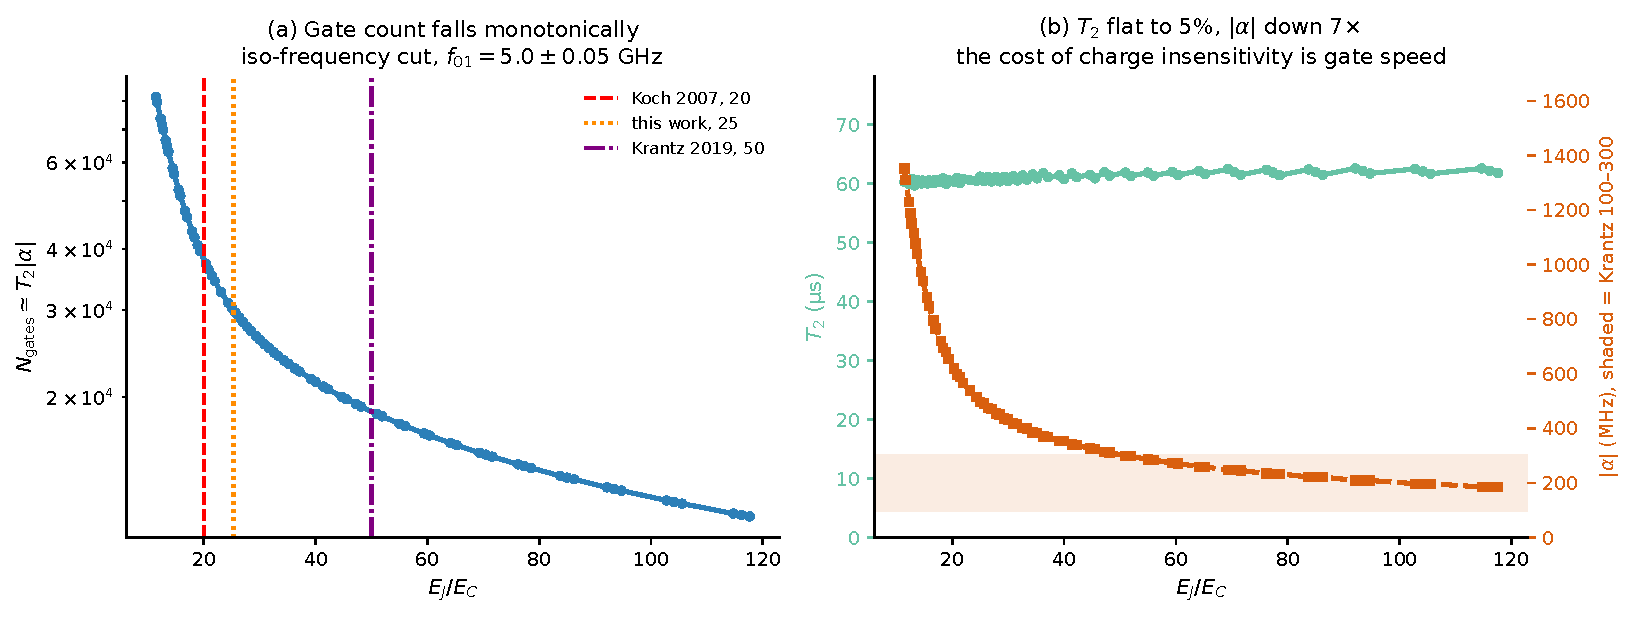
\includegraphics[width=\textwidth]{figures/transmon_tradeoff.pdf}
\caption{The transmon trade-off at fixed frequency ($f_{01} = 5.00 \pm
\SI{0.05}{\giga\hertz}$). (a) Gate count falls monotonically with $E_J/E_C$; the three
vertical lines are candidate regime thresholds, and the optimum sits on whichever one is
imposed. (b) $T_2$ is flat to 4.8\% while $|\alpha|$ falls $7.3\times$; the shaded band is
the Krantz \SIrange{100}{300}{\mega\hertz} design window. Charge insensitivity costs gate
speed, not coherence.}
\label{fig:tradeoff}
\end{figure}

Holding $f_{01} = 5.00 \pm \SI{0.05}{\giga\hertz}$ and sweeping $E_J/E_C$ from 11.4 to 117.6,
$T_2$ is flat to 4.8\% (\SIrange{59.7}{62.6}{\micro\second}) while $|\alpha|$ falls by a
factor of 7.3 (\SIrange{1353}{185}{\mega\hertz}). \textbf{Charge insensitivity is bought with
anharmonicity---that is, with gate speed---and essentially not with coherence at all}
(Fig.~\ref{fig:tradeoff}).

That the trade is anharmonicity-for-charge-insensitivity is expected from Koch's asymptotics:
with $\alpha \simeq -E_C$ and $f_{01} \simeq \sqrt{8E_JE_C}$ held fixed, raising $E_J/E_C$
forces $E_C \propto (E_J/E_C)^{-1/2}$, predicting a factor 3.21 over our swept range against a
measured $E_C$ ratio of 3.47. The observed $7.3\times$ fall in $|\alpha|$ is steeper still
because $\alpha \simeq -E_C$ is asymptotic and fails at the low end: $|\alpha|/E_C = 2.29$ at
$E_J/E_C = 11.4$ against $1.09$ at $117.6$. The trade-off is therefore harshest exactly in the
low-$E_J/E_C$ corner that an unconstrained gate-count metric wants to select, which is an
independent reason to keep the design envelope.

Relocating the gate-count optimum under eight regime thresholds spanning $E_J/E_C = 15$ to
60, the optimum tracks every one of them to within 0.24. It sits \emph{on} the constraint,
never inside the domain. This is the signature of a constrained optimum, and it means the
substantive choice in this part of the design space is the threshold, not the optimization. The correct claim is a monotone trade-off terminated wherever the
regime boundary is drawn, and any quoted optimum is meaningful only together with its
threshold. We adopt the Krantz envelope ($E_J/E_C \ge 50$, $|\alpha| \in
[100,300]$\,MHz, $f_{01} \in [3,6]$\,GHz)~\cite{krantz2019} because it is independent of every
noise amplitude in the study, giving the operating point $E_J = \SI{13.0}{\giga\hertz}$,
$E_C = \SI{0.26}{\giga\hertz}$, $f_{01} = \SI{4.92}{\giga\hertz}$,
$T_2 = \SI{62.4}{\micro\second}$, $|\alpha| = \SI{299}{\mega\hertz}$.

A limitation of the model bears on this choice: \texttt{tphi\_1\_over\_f\_ng} covers $1/f$
dephasing only, and the broadband charge sensitivity that motivates Krantz's
$E_J/E_C \ge 50$ is absent. Left to itself the metric under-penalizes low $E_J/E_C$ and would
recommend $|\alpha| \approx \SI{728}{\mega\hertz}$, roughly $2.4\times$ what is fabricated.
The envelope is a constraint imposed on the model, not a result derived from it.

\section{The Fluxonium Design Plane}
\label{sec:fluxonium}

Over $E_J \in [3,15]$, $E_L \in [0.2,1.5]$\,GHz at $E_C = \SI{2.5}{\giga\hertz}$ and
$\Phi/\Phi_0 = 1/2$, the same confound appears: $\mathrm{corr}(\log T_2, \log f_{01}) =
-0.9973$. The unconstrained maximum, \SI{5427}{\micro\second}, sits at both grid edges at
$f_{01} = \SI{75}{\mega\hertz}$, where $\bar n_{\rm th} = 3.7$---thermally scrambled and
$2.3\times$ below the lowest published device. Constrained to the published band
\SIrange{0.17}{0.83}{\giga\hertz} the best design gives \SI{2412}{\micro\second} at
$E_J = 11.8$, $E_L = \SI{0.405}{\giga\hertz}$.

\subsection{An interior optimum, created by second-order dephasing}

Extending the scan to $E_J = \SI{45}{\giga\hertz}$ reveals a genuine interior maximum in
$T_2$, present at every $(E_C, E_L)$ combination tested (Fig.~\ref{fig:interior}). It is created by the second-order
flux channel: as $E_J$ rises and $E_L$ falls the qubit sinks into a deep double well,
$f_{01}$ collapses, and $\partial^2 f_{01}/\partial\Phi^2$ grows by three orders of
magnitude across the scan, so $\Gamma_\Phi^{(2)}$ grows with it and eventually overwhelms the
improving dielectric $T_1$. At the turning point that channel carries 43--58\% of the total
dephasing rate, which is the signature of a genuine internal optimum: the channel that turns
the curve over is comparable to everything else exactly at the turn. A first-order-only
pipeline shows no turnover over the same range and rises monotonically, reaching
$4.2\times10^{5}$\,\si{\micro\second} at the end of the scan---which is precisely how an earlier version of this
analysis concluded there was no interior optimum, and is a concrete argument for including the
second-order channel in any design study that sweeps toward low $E_L$.

The mechanism is geometric. As $E_J$ rises and $E_L$ falls the potential minima separate and
the tunnel splitting that sets $f_{01}$ collapses; the same deepening well sharpens the
curvature to which $\Gamma_\Phi^{(2)}$ is proportional by Eq.~\eqref{eq:secondorder}, so a
single geometric change both lowers the frequency and raises the second-order rate. The
transmon has no analog: its charge dispersion falls
exponentially in $\sqrt{E_J/E_C}$ with no turning point.

\begin{figure}[t]
\centering
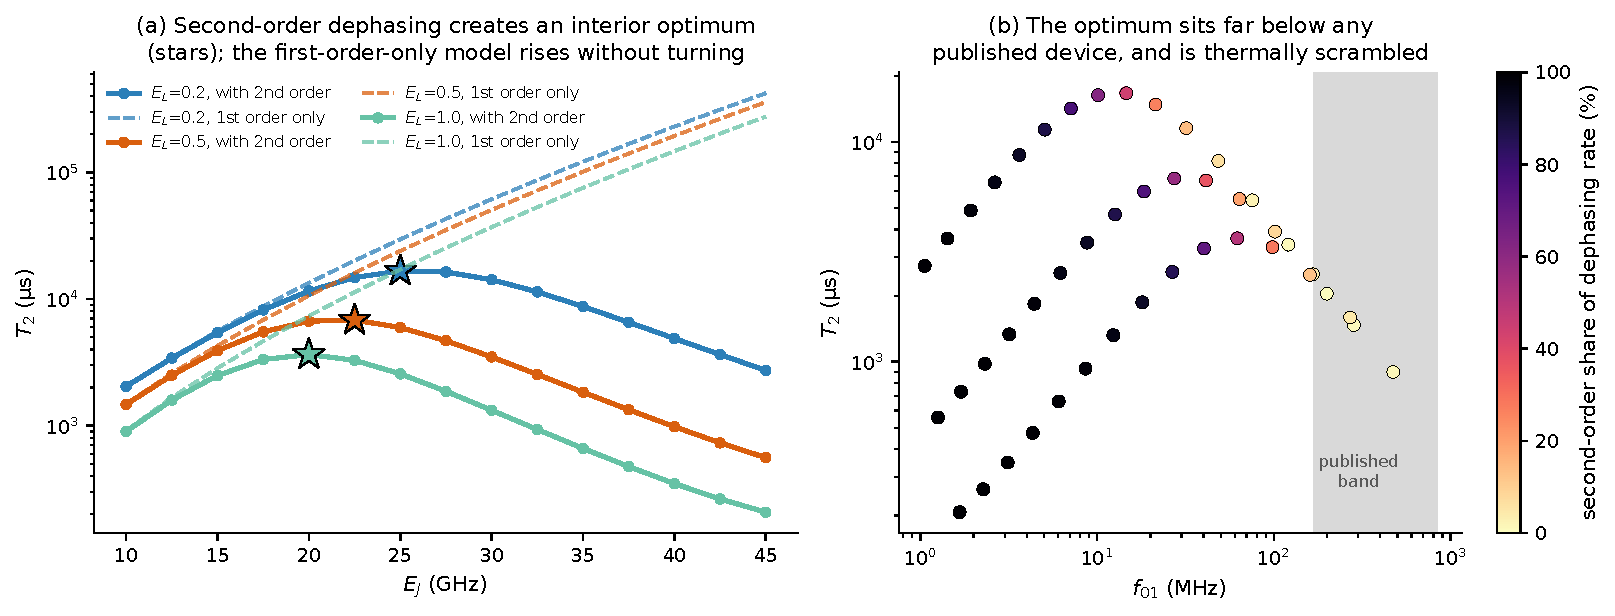
\includegraphics[width=\textwidth]{figures/fluxonium_interior_optimum.pdf}
\caption{(a) $T_2$ versus $E_J$ at three values of $E_L$. Solid curves include second-order
flux dephasing and turn over (stars); the dashed first-order-only curves rise without limit
over the same range, which is how the interior optimum was previously missed. (b) The same
points against $f_{01}$, colored by the second-order share of the dephasing rate. Every
turning point lies far below the published fluxonium band (shaded).}
\label{fig:interior}
\end{figure}

The optimum is nevertheless inaccessible. It occurs at $f_{01} = 10$--\SI{73}{\mega\hertz}
with $\bar n_{\rm th} = 4$--32. Past the turnover the frequency correlation reverses sign,
which is a further indication that the second-order channel introduces genuinely new
structure rather than rescaling the old.

\section{Dominant Noise Channels}

At a charge-sensitive bias ($n_g = 0.25$) charge noise dominates the transmon below
$E_J/E_C \approx 25$ and dielectric relaxation above it. That crossover is measured from our
own data and lands close to Koch's independently derived bound of 20; the two arguments are
unrelated---one a noise-budget crossover, the other a pulse-duration requirement---so their
agreement is genuine corroboration. Critical-current noise never dominates anywhere in 1600
points at literature amplitudes. The crossover is noise-model dependent (it spans 20.8--29.9
across literature ranges) and is therefore reported as a result rather than used as an input.

For the fluxonium, relaxation dominates at the sweet spot and first-order flux noise becomes
the largest single term beyond $2.75\times10^{-5}\,\Phi_0$. Quasiparticle tunneling is not a
dead channel: it is suppressed only \emph{at} the sweet spot, where its $0$--$1$ matrix
element vanishes by symmetry, and limits $T_1$ at most detuned points. This finding is
conditional on $x_{qp} = 3\times10^{-6}$, a default roughly $300\times$ above the bound of
$10^{-8}$ that Nguyen \emph{et al.} infer for their devices; at their density the channel is negligible everywhere. It is the
most fragile result in the study and is reported as conditional.

\section{The Cross-Architecture Comparison}

\subsection{Bias robustness, the one unambiguous asymmetry}

Both bias coordinates are periodic with period one, so the width of the window over which
$T_2$ stays within a factor $k$ of its sweet-spot value, as a fraction of one bias period, is
directly comparable. The transmon's $T_2$ varies by $1.0056\times$ across its \emph{entire}
charge period---a factor-of-two loss never occurs at any bias. The fluxonium loses a factor
of two within $\pm 3.61\times10^{-5}\,\Phi_0$ and a factor of ten within
$3.25\times10^{-4}\,\Phi_0$, located by root-finding on the model rather than read off a
grid. The usable bias window differs by $1.4\times10^{4}$.

The falloff exponent is not a single number. It approaches the first-order $1/f$ prediction
of $-1$ only in an intermediate window where $T_2$ is genuinely flux-dephasing limited,
reaching $-0.956$ there, and flattens on both sides---capped by the $2T_1$ ceiling close in,
and contaminated by other channels far out.

Intrinsic $1/f$ flux noise does not by itself drive the qubit off the spot: even at Nguyen's
measured amplitude integrated over an hour, the RMS wander leaves a $24\times$ margin to the
tenfold-loss detuning. The binding constraint is systematic drift and bias-line calibration,
not stochastic noise---which relocates the difficulty rather than removing it, and makes it
scale with qubit count.

\textbf{This constraint is being engineered away, which we should say plainly.} B\'en\^atre
\emph{et al.} hold gradiometric fluxonium qubits at their sweet spot passively, reporting
stability of $3\times10^{-4}\,\Phi_0$ from target with only a 15\% reduction in echo
coherence~\cite{benatre2025}. Their achieved stability sits essentially at our computed
tenfold-loss detuning of $3.25\times10^{-4}\,\Phi_0$, yet they observe far less degradation
than that number would suggest---unsurprisingly, since their device has different $E_L$ and
hence different curvature, and echo suppresses low-frequency drift that free induction does
not. We read their result as evidence that the bias-precision cost we quantify is real,
understood, and addressable by design rather than by calibration alone. It weakens the
scalability pessimism in our conclusion without touching the arithmetic behind it.

\subsection{No single ratio}

Table~\ref{tab:q3} gives the comparison under every metric we consider defensible, and
Fig.~\ref{fig:robust} shows how each fares across the noise band.

\begin{table}[t]
\caption{Fluxonium/transmon ratio by metric. MC = median over $N=400$ log-uniform draws of
each noise amplitude across its literature decade, with the 5--95\% sample spread.}
\label{tab:q3}
\centering
\begin{tabular}{@{}lccc@{}}
\toprule
Metric & Det. & MC med.\ [5--95\%] & Wins\\
\midrule
Raw $T_2$                       & $18.1$      & $11.3$ [3.6, 21.1]   & 100\%\\
$T_2$, matched $f_{01}$         & $1.1$--$2.2$ & $\mathbf{0.86}$ [0.27, 1.6] & \textbf{42\%}\\
Gates, $1/|\alpha|$             & $524$       & $326$ [104, 611]     & 100\%\\
Gates, $1/\min(|\alpha|,f_{01})$ & $22.0$     & $13.7$ [4.4, 25.6]   & 100\%\\
Gates, $1/f_{01}$               & $\mathbf{1.34}$ & $\mathbf{0.83}$ [0.26, 1.6] & \textbf{40\%}\\
Gates, simulated                & $48$        & --                   & --\\
\midrule
Bias window, $2\times$ loss     & \multicolumn{3}{c}{$1.4\times10^{4}$ wider for the transmon}\\
\bottomrule
\end{tabular}
\end{table}

Two ranges are visible, and they are of comparable size. \emph{Across} metrics the answer
spans roughly $500\times$ ($524\times$ against $1.07\times$, Table~\ref{tab:q3}). \emph{Within} the gate-count metric alone it spans $393\times$,
depending on what bounds the minimum pulse length. The $|\alpha|$ bound---leakage to
$|2\rangle$ only---is the textbook choice, but for a fluxonium at half flux
$|\alpha| = \SI{8.7}{\giga\hertz}$ is $24\times$ the transition frequency it would drive, so
that bound licenses a pulse $24\times$ shorter than one period of the transition itself. The
drive-period bound $1/f_{01}$ is equally physical and gives $1.34\times$.

\begin{figure}[t]
\centering
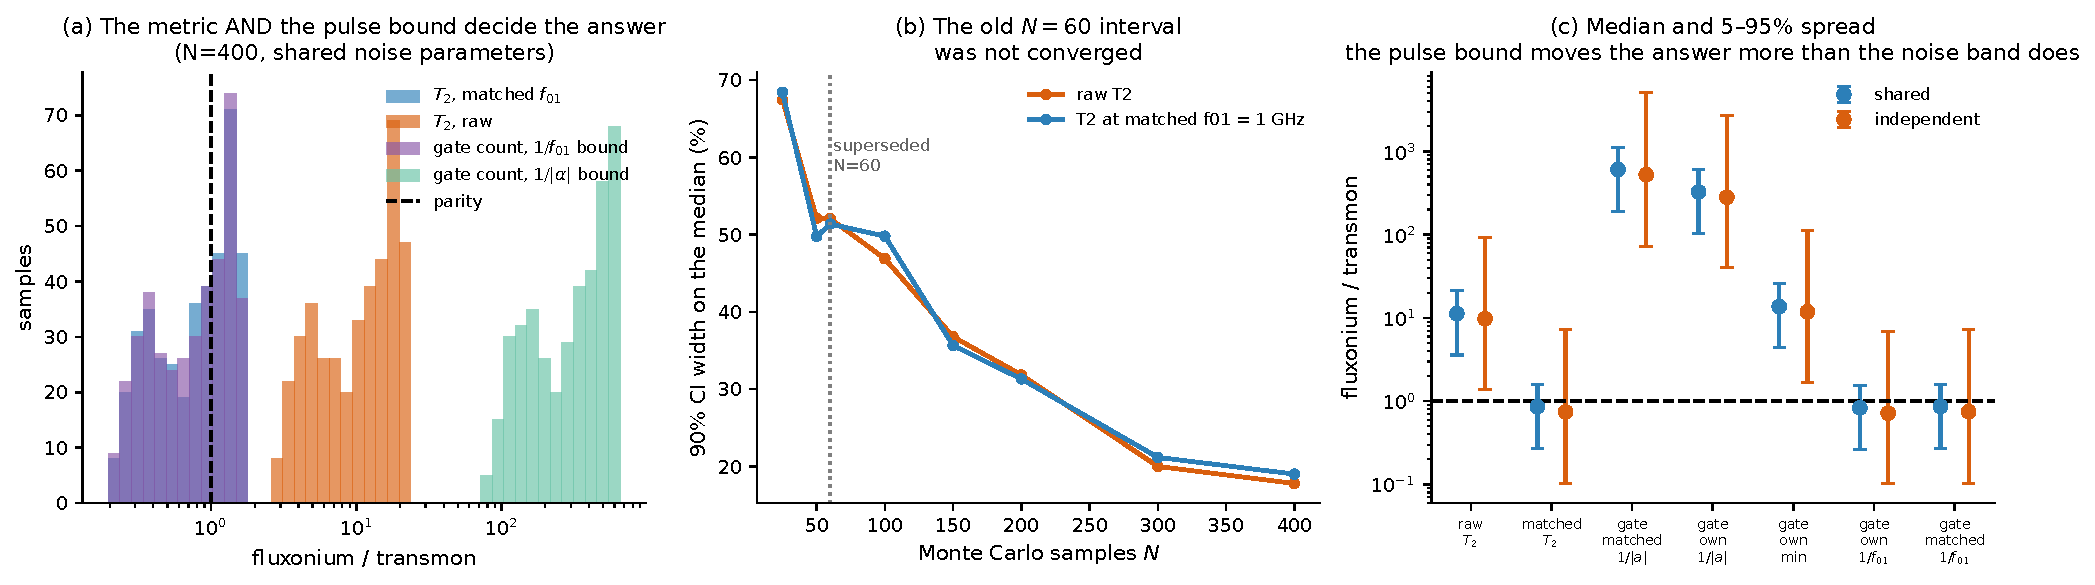
\includegraphics[width=\textwidth]{figures/q3_robustness.pdf}
\caption{Robustness of the Q3 answer to the noise amplitudes. (a) Distribution of the
fluxonium/transmon ratio under four metrics, $N=400$ shared-parameter draws; the metric and
the pulse bound each move the answer by more than the noise band does. (b) The 90\%
bootstrap CI on the median against sample size, showing that an earlier $N=60$ interval had
not converged. (c) Median and 5--95\% spread per metric under shared versus independent
sampling.}
\label{fig:robust}
\end{figure}

\subsection{The raw advantage is mostly frequency}

The two devices differ in frequency by $13.6\times$, and
$\log 13.55/\log 18.10 = 0.90$: about 90\% of the log-advantage is the frequency difference.
This is not a coincidence of these two designs. Dielectric loss dominates both architectures
and its rate scales with $\omega_{01}$, so $T_2 \propto 1/f_{01}$ in both---measured as
$f_{01}^{-0.965}$ for the transmon. Because the flux sweet spot \emph{is} a frequency
minimum, the fluxonium is structurally advantaged on any uncontrolled $T_2$ comparison, and
reporting one credits the architecture with what the frequency did.

Controlling for it, the deterministic ratio at matched $f_{01}$ is 1.07--2.16$\times$. But
propagated across the literature noise band the median is $0.86\times$ and the fluxonium wins
in only 42\% of samples. \textbf{At matched frequency the transmon is more often the better
device.} This is the most important negative result here: what remains of the coherence
advantage after the frequency control does not survive the noise-amplitude uncertainty.

\subsection{Settling the pulse bound}
\label{sec:pulse}

The gate-count range is wide enough to make the metric almost uninformative, so we settle it
by simulation rather than by argument. We integrate the lab-frame Schr\"odinger equation for
each architecture with no rotating-wave approximation, using a six-level truncation of the
\texttt{scqubits} eigenbasis and a charge drive, and calibrate each gate as an experimentalist
would: amplitude, DRAG coefficient~\cite{motzoi2009} and Stark-shifted drive frequency are
optimized at every duration, and the average gate error is evaluated on the computational
subspace so that leakage is counted; Fig.~\ref{fig:pulse} shows the resulting error curves.

This exposes an effect that the anharmonicity argument misses entirely. The fluxonium's
$|\alpha|/f_{01} = 24$ looks decisive, but its drive matrix elements are unfavourable: at
half flux $|\langle 1|\hat n|2\rangle| / |\langle 0|\hat n|1\rangle| = 10.2$, against $1.37$
for the transmon. The drive couples ten times more strongly to the leakage transition than to
the qubit transition, so the effective figure of merit is the anharmonicity divided by that
ratio, not the anharmonicity itself.

Table~\ref{tab:pulse} reports the shortest calibrated gate reaching an average error below
$10^{-3}$ for each architecture, and the resulting gate count. \emph{These durations are upper
bounds}: a three-parameter calibration over a fixed Gaussian shape is far from optimal
control, and GRAPE or CRAB over a free pulse shape would shorten both---not necessarily
equally. The point is not the precise value but that the simulated ratio falls decisively
between the two naive bounds, excluding both.

\begin{table}[t]
\caption{Shortest calibrated $X$ gate reaching an average error below $10^{-3}$, from the
lab-frame simulation, and the resulting gate count $N = T_2/T_{\rm gate}$. Durations are
upper bounds and are bracketed by the duration grid and by optimizer convergence.}
\label{tab:pulse}
\centering
\begin{tabular}{lccc}
\toprule
 & $T_{\rm gate}$ (ns) & $T_2$ (\si{\micro\second}) & $N$\\
\midrule
Transmon  & $8.0$ ($6.0$--$8.0$)  & $62.4$   & $7{,}803$\\
Fluxonium & $3.0$ ($2.5$--$3.0$) & $1129.7$ & $376{,}571$\\
\midrule
\multicolumn{3}{l}{\textbf{Simulated ratio}} & $\mathbf{48\times}$\\
\multicolumn{3}{l}{\quad bracket from grid + optimizer} & $36$--$58\times$\\
\multicolumn{3}{l}{\quad for comparison, $1/|\alpha|$ bound} & $524\times$\\
\multicolumn{3}{l}{\quad for comparison, $1/f_{01}$ bound} & $1.34\times$\\
\bottomrule
\end{tabular}
\end{table}

The result is that the fluxonium does convert coherence into operations more efficiently than
the transmon, but by a factor of order $36$--$58\times$ rather than the ${\sim}500\times$ the anharmonicity bound suggests or the ${\sim}1\times$ the drive-period bound suggests. Neither extreme survives contact with a simulated pulse, and the residual uncertainty is dominated by optimizer convergence rather than by physics.

\begin{figure}[t]
\centering
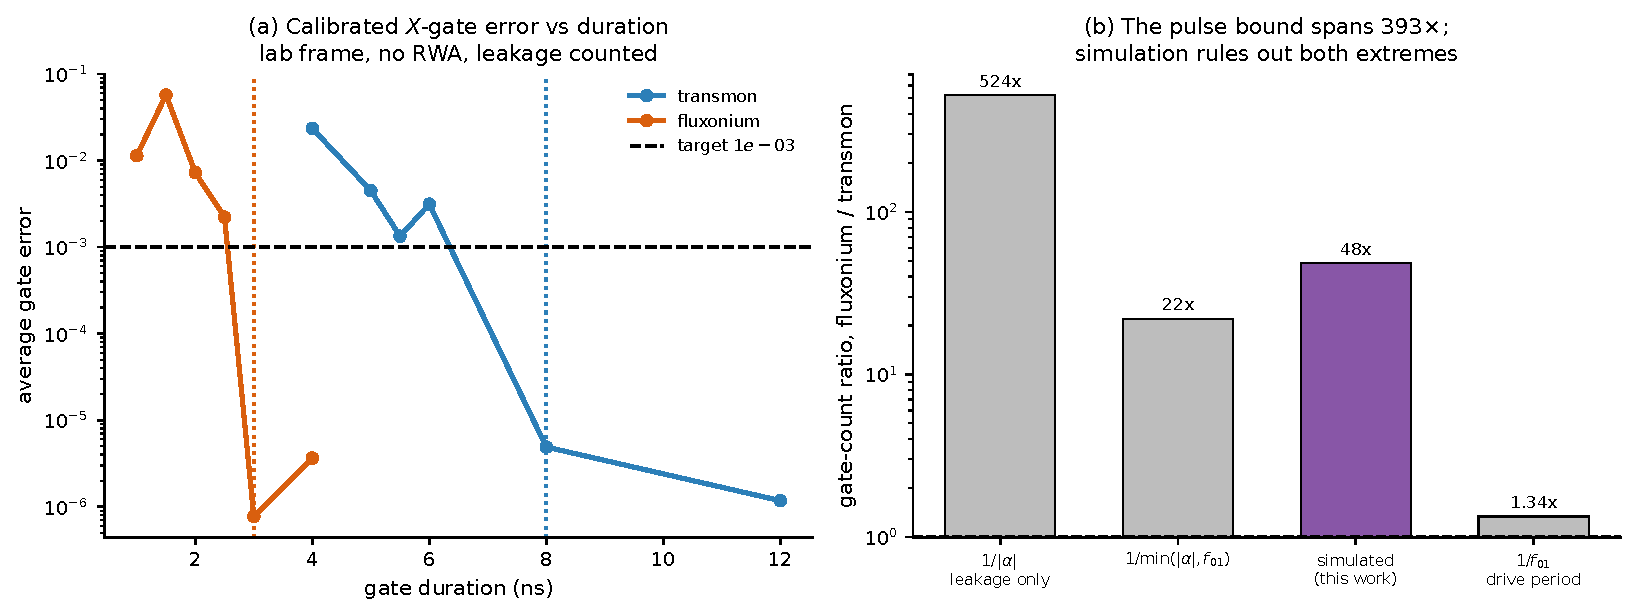
\includegraphics[width=\textwidth]{figures/q3_pulse_bound.pdf}
\caption{(a) Average $X$-gate error against gate duration for both architectures, from the
lab-frame simulation with amplitude, DRAG and Stark detuning calibrated at each point;
dotted lines mark the shortest duration meeting the $10^{-3}$ target. Non-monotonicity at the
shortest durations is optimizer noise and is not smoothed. (b) The gate-count ratio under
each pulse-length bound. The two analytic bounds differ by $393\times$; the simulation
(purple) falls between them and excludes both.}
\label{fig:pulse}
\end{figure}

\section{Calibration Against Measurement}
\label{sec:calibration}

Run at the parameters of each of the nine devices in the published Table~I of Nguyen
\emph{et al.}, the model is optimistic by a median factor of $2.0\times$ on $T_1$ and
$2.6\times$ on $T_2$, worst case $5.7\times$. The gap is not uniform, so it is not a single
missing constant---and it is smallest where it matters most: device~I, the device nearest our
nominal design in frequency (0.395 versus \SI{0.363}{\giga\hertz}), is matched to 4\% on
$T_2$, with the model \emph{pessimistic} on its $T_1$.

Identified contributors, in order: the flat $Q_{\rm cap} = 10^6$ against their measured
$\tan\delta_C = (2.0$--$3.6)\times10^{-6}$ at \SI{6}{\giga\hertz}; the absence of Purcell
decay, photon shot noise and inductive loss; the fact that their $T_2$ is a Hahn echo while
this model computes free-induction decay, which makes the comparison conservative in the
model's favor; and a temperature mismatch, since we run at the \SI{15}{\milli\kelvin}
default while they state \SI{20}{\milli\kelvin}.

The comparison also has a floor set by our own model rather than by the devices. Absolute
$T_2$ spans \SIrange{149}{3316}{\micro\second} under single-decade moves of the noise
amplitudes, so a factor of $2.6$ is well inside the band the model itself admits; the
calibration should be read as establishing the right order of magnitude, not as a residual to
be explained away. Consistent with that, the state of the art has moved well past the devices
we calibrate against---Somoroff \emph{et al.} report $T_2^* = 1.48$\,ms~\cite{somoroff2023}, so
a model tuned to reproduce Nguyen's 2019 numbers exactly would now be miscalibrated against
2023 hardware.

We stress that the published table must be used. The arXiv v1 preprint lists eight devices
and omits device~I entirely---the paper's headline device, and the one closest to the design
regime studied here.

\section{Limitations}
\label{sec:limitations}

The model omits Purcell decay, photon shot noise, inductive loss in the junction array, TLS
spectral structure, crosstalk and any lattice; qubits are treated in isolation. The
superinductance is ideal, so array-mode hybridization is absent, though
Section~\ref{sec:validation} bounds that omission at $-0.43\%$ in $f_{01}$ at the flux sweet
spot. Second-order dephasing uses a convention with no logarithmic factor; a $\ln^2$
convention would change sweet-spot $T_2$ by ${\sim}37\%$ instead of 0.6\% and would move,
though not remove, the interior optimum. Absolute $T_2$ spans
\SIrange{149}{3316}{\micro\second} under single-decade moves of the noise amplitudes and
should never be quoted without a band. The Monte Carlo varies amplitudes only; fabrication
spread in $E_J$, $E_C$, $E_L$ is not propagated, and the log-uniform priors are a choice. The
gate-count metric is a heuristic, not a literature formula.

\section{Conclusion}

Neither architecture has a usable coherence sweet spot in design space. Both design planes are, to
better than $|r| = 0.99$, restatements of the transition frequency, so a raw $T_2$ maximum
locates the edge of the swept domain or the point where a frequency constraint was drawn.
The transmon is a monotone trade-off in which charge insensitivity is paid for in
anharmonicity, once, at design time. The fluxonium has a real interior optimum, visible only
once second-order flux dephasing is included, but it is thermally out of reach; in practice
it too is a trade-off terminated by a frequency floor.

For Q3, the honest output is a metric family, not a number. The fluxonium's raw $18\times$
coherence advantage is roughly 90\% frequency; at matched frequency it inverts to a median
$0.86\times$ across the literature noise band. Its durable advantage is anharmonicity per
unit coherence, and its price is operating-point precision---a bias window four orders of
magnitude narrower than the transmon's, paid continuously at run time rather than once at
design time. Whether that trade is worth making is a question about qubit count and
calibration budget, not about coherence.

More generally, we suggest that architecture comparisons in this field should state the
metric, the control variable and the uncertainty band together. A single ratio between two
architectures at their own operating points is not a comparison between architectures.

\section{Outlook}

Two extensions would sharpen the results most. The gate-count metric is currently settled by a
coarse calibration; optimal control over a free pulse shape (GRAPE or CRAB) would tighten the
$36$--$58\times$ bracket and, more interestingly, would test whether the fluxonium's
unfavourable leakage matrix element can be shaped around---the anharmonicity is genuinely
there, and a pulse that exploits it without driving $|1\rangle \to |2\rangle$ would move the
number back toward the leakage-only bound. Second, the interior fluxonium optimum we find is
thermally inaccessible at \SI{15}{\milli\kelvin}, but that is a statement about temperature as
much as about design; the same analysis at lower base temperature, or with active
initialization modeled, would establish whether it is inaccessible in principle or merely
inconvenient.

A broader point follows from the metric sensitivity. If a single architecture comparison can
span more than two orders of magnitude depending on choices that are all defensible, then comparisons
reported as single ratios carry less information than they appear to. We would encourage the
practice McRae \emph{et al.}~\cite{mcrae2021} advocate for experimental coherence
numbers---report the conditions with the number---to be extended to modeled design
comparisons: state the control variable, state the figure of merit, and give the spread.

\section*{Code and data availability}
\addcontentsline{toc}{section}{Code and data availability}

All code, generated data and figures are openly available at
\url{https://github.com/ishitabera/quantum-coherence-sweet-spots-transmon-fluxonium}.

Every number in this paper is produced by five notebooks run in order from a single validated
pipeline; no notebook reimplements the physics. Each sweep writes its raw data before any
figure code executes, together with a metadata record of the grid, the noise amplitudes, the
software versions and the git revision. Every quoted value is bound to the file and filter
that produced it by an automated provenance ledger of 33 entries, which recomputes and asserts
each one on every run and fails rather than warns if a value drifts from its artifact. A test
suite of 32 checks pins the conventions and the validated anchors, including the published
numbers used for calibration.

\section*{Acknowledgments}

\paragraph{Use of generative AI}
This work was carried out by the author together with a large language model (Claude,
Anthropic), which contributed to the analysis code and the numerical analysis. The author
wrote the manuscript with its assistance, reviewed it, double-checked the physics and the
numerical results, and is responsible for all claims.

\paragraph{Funding}
This work was carried out as a self-directed project and received no external funding.

\bibliography{refs}

\end{document}
